\documentclass[12pt, a4paper]{article}


\usepackage{microtype}
\usepackage{newpxtext, newpxmath}
\usepackage[T1]{fontenc}
\usepackage[margin=3cm]{geometry}
\usepackage{setspace}
  \setstretch{1.1}
\usepackage{amsmath}
\usepackage{bm}
\usepackage[dvipsnames]{xcolor}
\usepackage{fontawesome}
\usepackage{graphicx}
%\usepackage{pdflscape}
%\usepackage{rotating}
\usepackage{booktabs}
\usepackage{colortbl}
  \newcommand{\sampled}{\cellcolor{gray!20}}
\usepackage{placeins}
\usepackage[font=small, labelfont=bf]{caption}
\usepackage{hyperref}
  \hypersetup{
    colorlinks=true,
    linkcolor=BrickRed,
    filecolor=BrickRed,
    citecolor=BrickRed,
    urlcolor=RoyalBlue,
  }
\usepackage[capitalize, nameinlink]{cleveref}
\usepackage[figure]{hypcap}
\usepackage[super, comma]{natbib}
  \setlength{\bibsep}{0.2em plus 0.1em}
  \renewcommand{\bibfont}{\small}
\usepackage{authblk}
  \renewcommand\Affilfont{\itshape\normalsize}
\usepackage[disable]{todonotes}
\usepackage[left]{lineno}  % needed for Nature
%\linenumbers  % remove it for arXiv but keep it for journal submission


% journals
\newcommand{\mnras}{{\em Mon. Not. Roy. Astron. Soc. }}
\newcommand{\apjl}{{\em Astrophys. J. Let. }}
\newcommand{\apjs}{ApJS}
\newcommand{\jcap}{JCAP}
\newcommand{\nat}{{\em Nature}}
\newcommand{\physrep}{{\em Phys. Rept. }}
\newcommand{\aap}{{\em Astron. Astrophys. }}
\newcommand{\aj}{AJ }
\newcommand{\apj}{ApJ}
\newcommand{\pasp}{PASP}
\newcommand{\pasj}{PASJ}
\newcommand{\prl}{\em Phys. Rev. Lett. }
\newcommand{\ssr}{\em Space Sci. Rev.}
\newcommand{\araa}{Annual Review of Astron and Astrophys}
\def\prd{{\em Phys. Rev. }{\bf D }}
\def\pr{{Phys.\ Rev.\ }}
\def\astropart{{Astro-particle Phys.~}}
\def\rvmp{{Rev.\ Mod.\ Phys.\ }}

% useful commands
\bmdefine{\vtheta}{\theta}
\newcommand{\As}{A_\mathrm{s}}
\newcommand{\ns}{n_\mathrm{s}}
\newcommand{\Omegam}{\Omega_\mathrm{m}}
\newcommand{\Omegac}{\Omega_\mathrm{c}}
\newcommand{\Omegab}{\Omega_\mathrm{b}}
\newcommand{\OmegaL}{\Omega_\Lambda}
\newcommand{\zetaUV}{\zeta_\mathrm{UV}}
\newcommand{\HI}{\mathrm{HI}}
\newcommand{\He}{\mathrm{He}}
\newcommand{\HeII}{\mathrm{HeII}}
\newcommand{\e}{\mathrm{e}}
\newcommand{\re}{\mathrm{re}}
\newcommand{\reio}{\mathrm{reio}}
\newcommand{\rec}{\mathrm{rec}}
\newcommand{\ap}{\alpha}
\newcommand{\tilt}{\beta}
\newcommand{\ar}{\tilde{a}}
\newcommand{\gomp}{\mathrm{gomp}}

\newcommand{\paulo}[1]{{\bfseries\textcolor{cyan}{[PMC: #1]}}}
\newcommand{\PMCtodo}[2][]{\todo[backgroundcolor=Green!20, linecolor=Green!50, #1]{PMC: #2}}
\newcommand{\YL}[1]{\textcolor{Bittersweet}{\textbf{#1}}}
\newcommand{\YLtodo}[2][]{\todo[backgroundcolor=Bittersweet!20, linecolor=Bittersweet!50, #1]{#2}}


% title limited to 75 characters
\title{Five parameters are all you need\\(in $\Lambda$CDM)\vspace{2em}}


\author[1]{Paulo Montero-Camacho\thanks{\texttt{pmontero@pcl.ac.cn},
with equal contribution}}
\author[1]{Yin Li\thanks{\texttt{eelregit@gmail.com}, with equal
contribution}}
\author[2]{Miles Cranmer}
\affil[1]{Department of Mathematics and Theory, Peng Cheng Laboratory,
\newline Shenzhen, Guangdong, China}
\affil[2]{Institute of Astronomy, University of Cambridge, Madingley Road, Cambridge, UK\\
Department of Applied Mathematics and Theoretical Physics, University of Cambridge, Wilberforce Road, Cambridge, UK}


\date{}


\begin{document}


\maketitle


\paragraph{\large Abstract}  % 200 words

The standard cosmological model, with its six independent parameters,
has proven remarkably successful in describing the evolution of the
Universe.
One of these parameters, the optical depth to reionization $\tau_\reio$,
represents the scatterings that Cosmic Microwave Background (CMB)
photons will experience after decoupling from the primordial plasma as
the intergalactic medium transitions from neutral to ionized.
$\tau_\reio$ depends on the neutral hydrogen fraction $x_\HI$, which, in
turn, should theoretically depend on cosmology.
We present a novel method to establish the missing link between
cosmology and reionization timeline.
We discover the timeline has a universal shape well described by the
Gompertz mortality law, applicable to any cosmology within our simulated
data.
This enables us to map cosmology to reionization using
symbolic regression and to treat $\tau_\reio$ as a derived parameter.
Reanalyzing CMB data with our universal $x_\HI$ tightens the constraint
on $\tau_\reio$ by more than one order of magnitude to $\approx 1\%$ and
reduced the error on the amplitude of the primordial fluctuations by a
factor of 2.5 compared to Planck's PR3 constraint.
While our results rely on the astrophysical assumptions in our
simulations, the methodology itself is independent of these assumptions;
after all, $\tau_\reio$ is fundamentally a function of cosmology.

\newpage


% main article limited to 2500 words and 4 figures
\section*{Introduction}

% the separation of sections here is artificial, the body does not have an intro, results nor outro

The $\Lambda$CDM cosmological model has proven extremely effective in
predicting the evolution of our Universe, relying on only six parameters
\cite{Planck2020a}.
In particular, it explains the transition from a predominantly neutral
state in the early stages to the familiar ionized intergalactic medium
(IGM) observed in our relatively nearby surroundings.
This transition is known as cosmic reionization.
Despite a comprehensive understanding of the astrophysical principles
governing this transition, uncertainties persist regarding its precise
timeline \cite{Jin2023}.
The advent of the James Webb Space Telescope (JWST) \cite{Gardner2006}
represents a pivotal moment, substantially bolstering our ability to
directly constrain the evolution of the neutral hydrogen fraction
$x_\HI$.
This progress is being driven by the JWST's enhanced detection
capabilities, enabling the observation of high-redshift quasars
\cite{Eilers2023} and high-redshift galaxies
\cite{Adams2023, Bradley2023, Donnan2023}.

Reionization leads to scattering of Cosmic Microwave Background (CMB)
photons by free electrons, disrupting the CMB angular power spectra
($C_\ell$).
This scattering suppresses the signal at scales smaller than the Hubble
scale at reionization (approximately $\ell>10$) \cite{Planck2020b} due
to the optical depth $\tau_\reio$.
Additionally, it introduces a new signal in the polarization of CMB
photons at large angular scales \cite{Planck2020a}, that is $\propto
\tau_\reio$ in $C^{TE}_\ell$, the cross-correlation of the $E$-mode
polarization with the temperature (intensity), and is $\propto
\tau_\reio^2$ in $C^{EE}_\ell$, the $E$-mode polarization angular auto
power spectrum.
Consequently, heightened sensitivity to CMB polarization becomes crucial
for mitigating the degeneracy between $\tau_\reio$ and other
cosmological parameters, particularly $\As$, the amplitude of the
primordial scalar power spectrum, and $r$, the ratio of tensor-to-scalar
modes \cite{Natale2020}.

While the high-$\ell$ signal holds most of the constraining power for
cosmological parameters, the low-$\ell$ polarization is crucial for
accurately determining $\tau_\reio$, particularly through its impact on
$C^{EE}_\ell$.
Hence\YLtodo{connection not obvious to me}, \paulo{How about rephrase: the inclusion of low-$\ell$ -- polarization -- data leads to a lesser degeneracy between $\As$ and $\tau_\reio$ and can diminish the...?} be breaking the degeneracy with $\As$ and diminishing\YLtodo{can diminish?} the influence
of $\tau_\reio$ on other anomalous parameters like $A_\mathrm{lens}$
\cite{Giare2023}.
$A_\mathrm{lens}$ contains information about the expected deflection of
CMB photons due to the underlying matter distribution.
However, interpreting signals at large angular scales (low $\ell$)
without affecting high-$\ell$ measurements has proven challenging.
\YLtodo[inline]{need to ask Paulo more about these 2 sentences.}
This challenge may ultimately require adopting a comprehensive Bayesian
framework to jointly consider cosmology, astrophysics, and instrument
systematics \cite{Paradiso2023}.
\Cref{fig:tau} illustrates current representative constraints on
$\tau_\reio$ \paulo{This paragraph, which should be connected to the ``While...'' but due to the inline comment looks like a separate paragraph, is addressing $\tau_\reio$ measurements/challenges, I feel it is okay.}.\YLtodo{feels a bit out of place here}

\begin{figure}[tb]
\centering
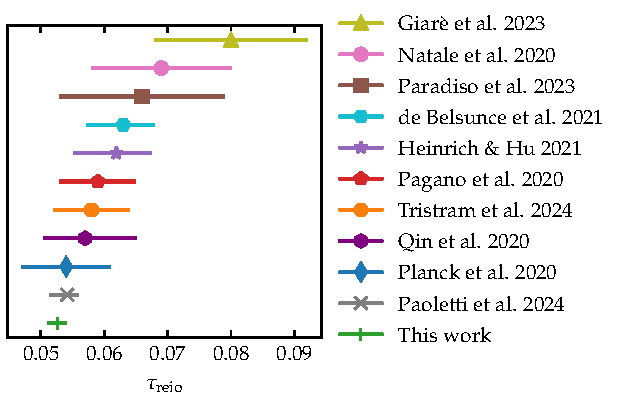
\includegraphics{figs/tau_fig.pdf}
\caption{\textbf{Current constraints on the optical depth to
reionization ($\tau_\reio$) from Cosmic Microwave Background (CMB)
data.}
The error bars indicate the 1$\sigma$ uncertainties.
Various analyses may employ distinct data sets or vary in the parameters
considered.
For instance, the inclusion of WMAP data in Refs.~ \cite{Natale2020,
Paradiso2023} (circle and square) or ACT in combination with other
external data sets \cite{Giare2023} (triangle), expanded sky coverage
\cite{Paradiso2023} (square), incorporation of high-$\ell$ data
\cite{Pagano2020, Planck2020a, Giare2023} (pentagon, star, and
triangle), marginalization over small set of strongly correlated
parameters \cite{Natale2020} (circle), and the implementation of an
end-to-end Bayesian framework that marginalizes over astrophysics and
instrumental systematics \cite{Paradiso2023} (square).}
\label{fig:tau}
\end{figure}

Given the challenges posed by $\tau_\reio$ in CMB analyses and the
anticipated advancements in constraining the reionization timeline
\cite{Montero2021, Hera2022}, now is an opportune moment to reassess its
role.
In theory, cosmic reionization is uniquely determined given a specific
cosmology, i.e.\ by the other five cosmological parameters.
Specifically, the evolution of the global fraction of neutral hydrogen
can be written as
%
\begin{equation}
\label{eq:premise}
x_\HI(a) = f(a; \sigma_8, \ns, h, \Omegab, \Omegam)
\quad \Rightarrow \quad
\tau_\reio = g(\sigma_8, \ns, h, \Omegab, \Omegam),
\end{equation}
%
where $\ns$, $h$, $\Omegab$, and $\Omegam$ are the tilt of the
primordial power spectrum, dimensionless Hubble constant, and present
baryon and matter densities, respectively.
$\sigma_8$ is the present linear rms relative density fluctuation in a
sphere of radius $8 \, h^{-1}\mathrm{Mpc}$.
This parametrization chosen for convenience fully determines $x_\HI$,
but the incomplete understanding of cosmic reionization obscures this
mapping, necessitating the introduction of $\tau_\reio$ in CMB analyses.
However, our understanding of the astrophysical processes governing
reionization has significantly improved \cite{Gnedin2022, Kannan2022,
Murray2020, Fan2023} since the inclusion of $\tau_\reio$ became a
standard practice.
Ongoing and forthcoming observations promise to further our
understanding and reduce inherent modeling uncertainties.
Motivated by these developments, we use symbolic regression (SR)
\cite{Cranmer2023} to construct a mapping between cosmology and
reionization timeline, aiming to demote $\tau_\reio$ from an independent
to a derived cosmological parameter.

Accurately measuring the optical depth to reionization could
significantly tighten cosmological parameter constraints, especially as
$\tau_\reio$ remains the only independent cosmological parameter not
constrained to sub-percent precision \cite{Planck2020b}.
To achieve this precision, sensitivity to E-mode polarization at levels
$\lesssim 10^{-2} \, \mu$K$^2$ and meticulous control of systematic
effects and foregrounds residuals are essential.

\cref{eq:premise} introduces a novel avenue to constrain cosmology
by examining the dependence of $x_\HI(z)$ on cosmological parameters.
This mapping can enhance parameter constraints and shed light on
reionization astrophysics.
It also aids ongoing efforts in parametrizing cosmic reionization models
\cite{Trac2018, Trac2022} by including the cosmological dependence of
$x_\HI$.


\section*{Results}

Here, we present a universality in the neutral hydrogen time evolution,
and derive through SR its dependence on cosmology on simulated
reionization histories from \texttt{21cmFAST} \cite{Murray2020}.
We integrate this shape into \texttt{CLASS} \cite{Blas2011}, a popular
Boltzmann solver for CMB analyses.
We then evaluate the modified \texttt{CLASS} alongside \texttt{Cobaya}
\cite{Torrado2020}, a speed-aware sampler\cite{Lewis2002,
Lewis2013}\footnote{With adaptive covariance learning and fast-dragging
as in \cite{Neal2005}, enabling larger steps in slow parameters via
intermediate transitions of fast parameters.}, showcasing its ability to
recover parameter constraints from CMB data, including `TTTEEE' +
lensing likelihoods \cite{Planck2020c, Planck2020d} (see \Cref{fig:tg}).
Finally, we demonstrate cosmological gains by computing $\tau_\reio$ as
a derived parameter using our approach -- \cref{eq:premise} --
compared to sampling over $\tau_\reio$ using the conventional $\tanh$
model \cite{Lewis2008}.
We summarize our strategy in \Cref{fig:big}.

\begin{figure}[tb]
\centering
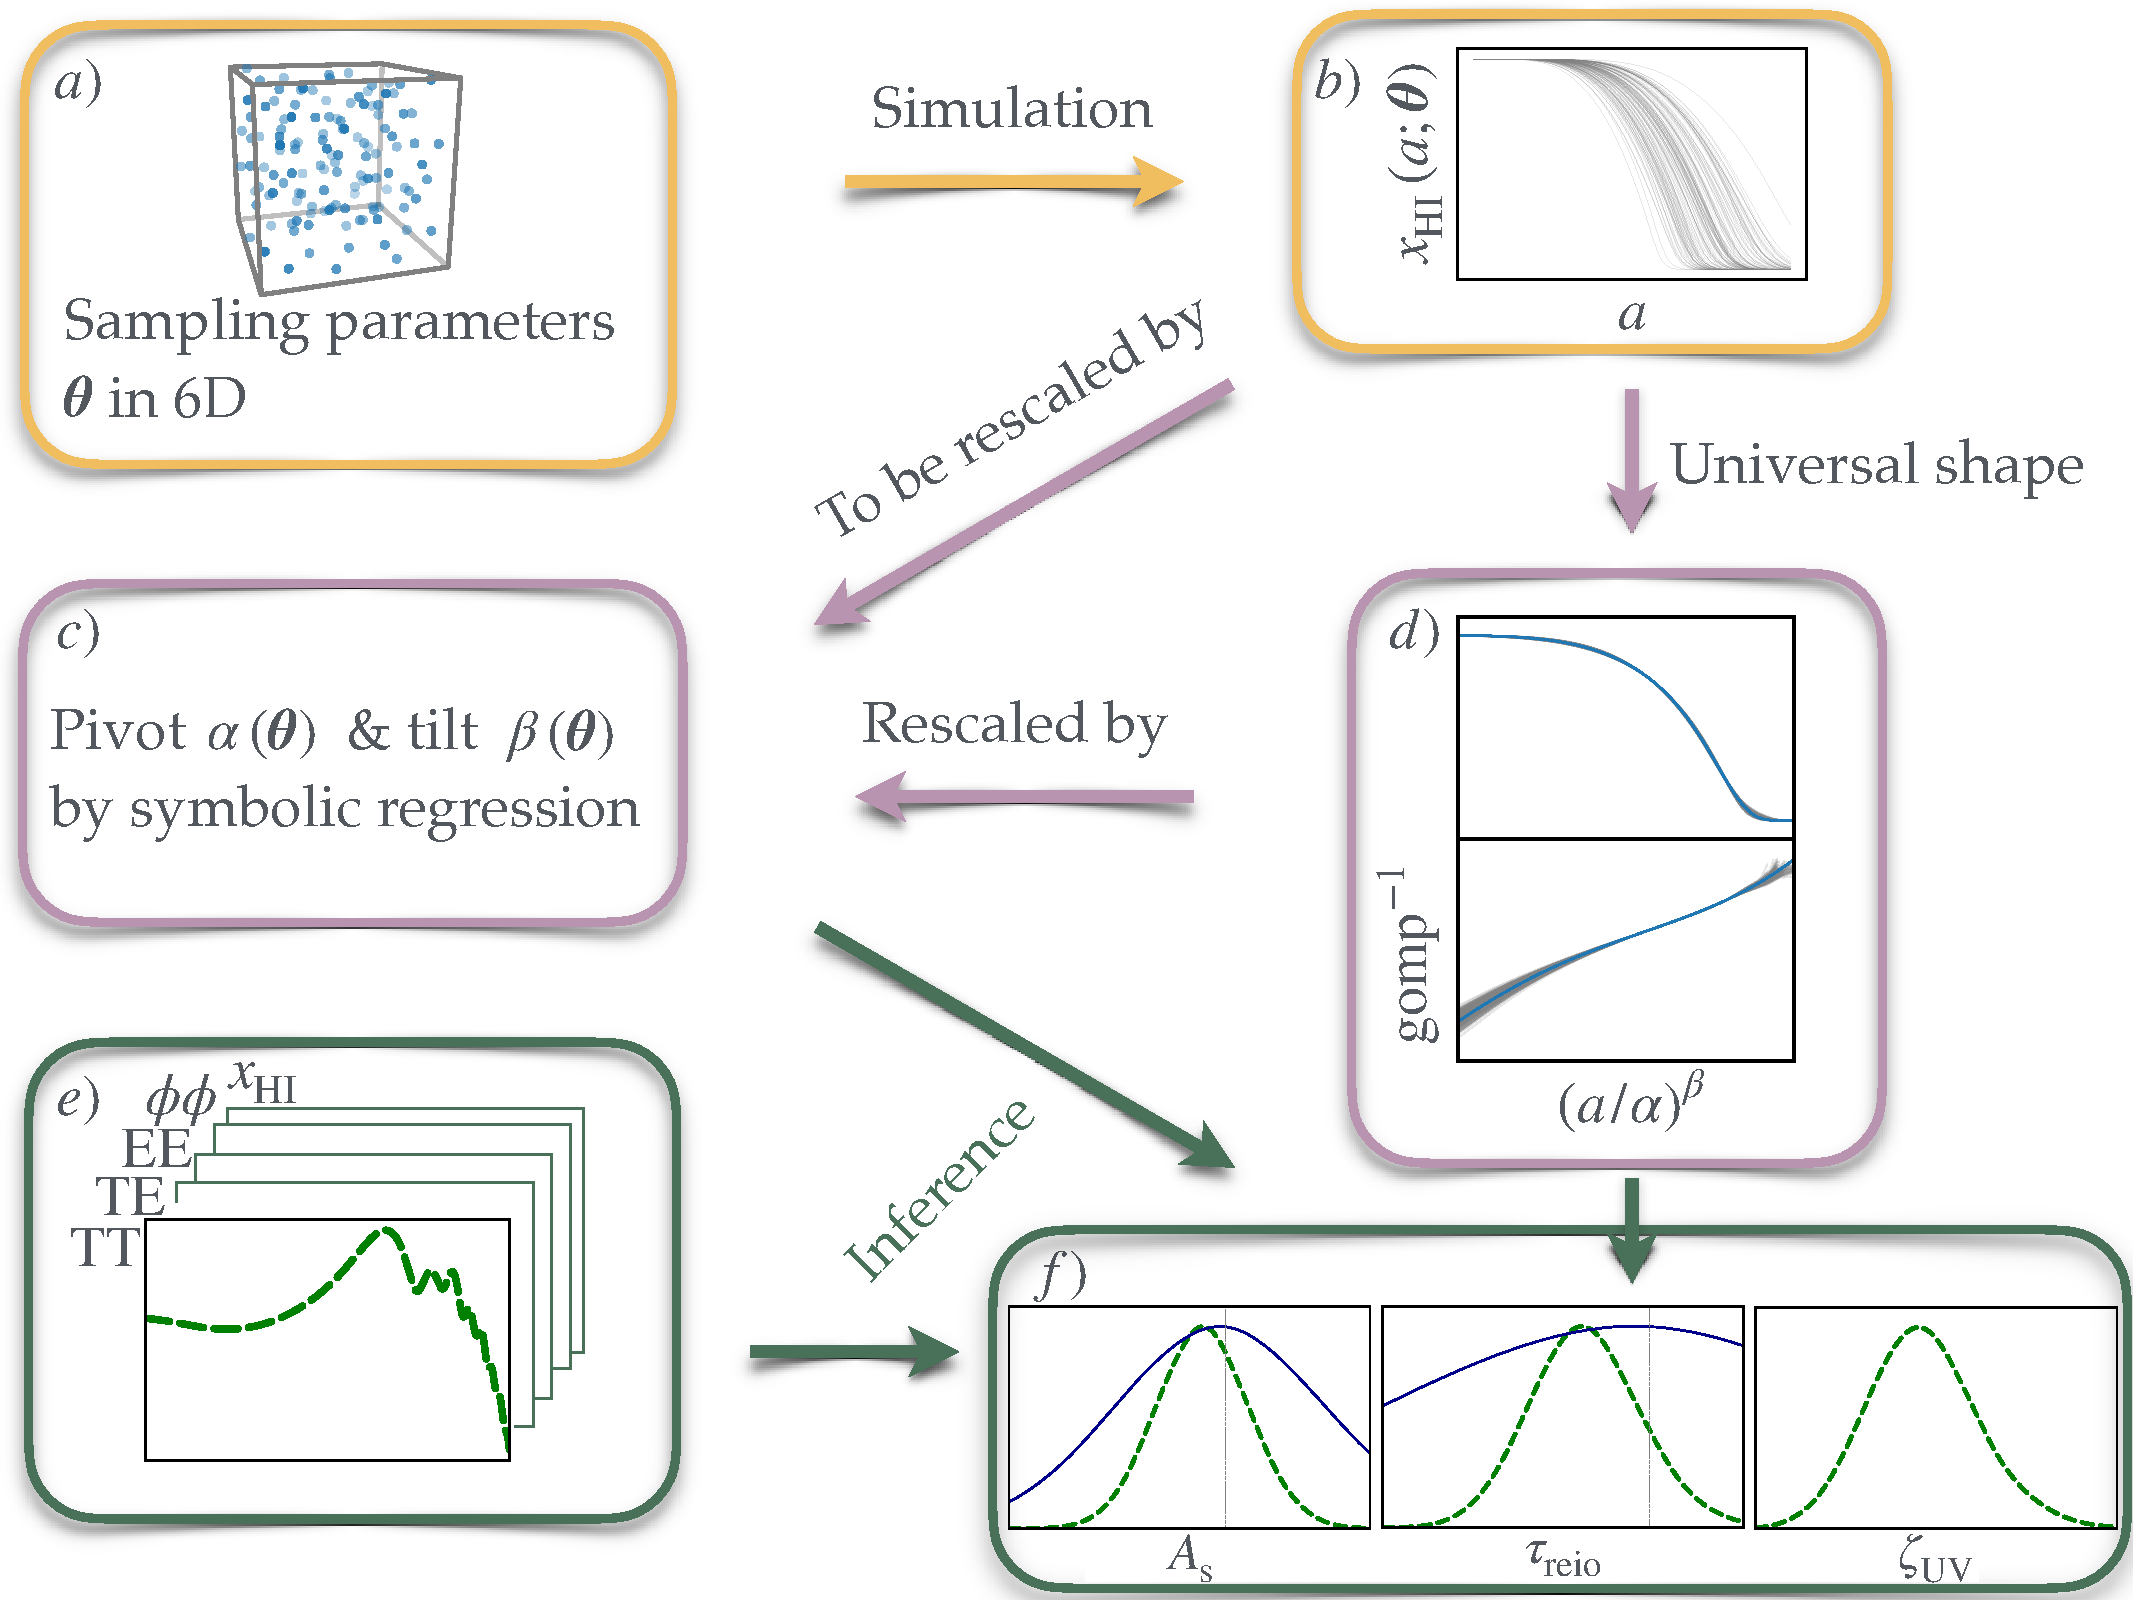
\includegraphics[width=\linewidth]{figs/big_fig.pdf}
\caption{\textbf{Strategy to demote $\tau_\reio$ to derived parameter.}
\emph{a)} Sobol sampling of $\vtheta$ comprising 5 cosmological and 1
astrophysical parameters (see \Cref{fig:sobol} in Extended Data).
\emph{b)} Simulated $x_\HI$ timelines as a function of $\vtheta$ and
scale factor $a$.
\emph{c)} With symbolic regression, we optimize the mapping from
$\vtheta$ to the rescaling parameters that bring the universality.
\emph{d)} We model the universal shape (upper panel) as a composition of
the Gompertz function and a low-degree polynomial (lower panel).
\emph{e)} Planck CMB data we re-analyze.
\emph{f)} We infer the parameter constraints using Monte Carlo Markov
Chain.}
\label{fig:big}
\YLtodo[inline]{Now we need to change to inverse \textbf{g}omp. Sorry...}
\end{figure}

To achieve our goal outlined in \cref{eq:premise}, we construct a
universal shape for $x_\HI$.
All $x_\HI(a)$ profiles share this shape, with differences between
scenarios being mere translations and rescalings.
Reionization causes $x_\HI$ to reduce from near 1 to effectively 0 via a
sigmoid transition.
The standard $\tanh$ function is symmetric in nature and not flexible
enough to provide the early start and rapid completion suggested by
reionization simulations \cite{Trac2018, Doussot2019}.
The Gompertz curve, an asymmetric sigmoid function often used to analyze
age-dependent human mortality \cite{Gompertz1825}, proves a good model
the survival of neutral hydrogen too.
Its expected accelerated increase in mortality with age resembles the
expectation for the percolation of ionized HII bubbles during the end
stages of reionization.

One way to uncover the universality is to view each $x_\HI$ scenario as
a cumulative probability distribution (CDF) in $- \ln a$.
With this insight, we can translate and rescale each timeline using the
mean and variance of its corresponding probability density function
(PDF), i.e.\ $- \mathrm{d}x_\HI / \mathrm{d}\ln a$, and discover the
existence of a universal shape followed by all scenarios.
Therefore, cosmology only impacts the translation and rescaling
parameters of each timeline, not its shape.

However, with the PDF trick, some $x_\HI$'s can deviate artificially
from universality, due to their incomplete reionization given our broad
range of simulated scenarios.
To address this, we adopt a better approach to jointly fit the global
shape and the 2 individual parameters of each $x_\HI$.
Our shape model constitutes the Gompertz function composed with a
5th-degree polynomial, in the translated-and-rescaled time $\ln\ar
\equiv \tilt (\ln a - \ln\ap)$.
And we are free to set the polynomial constant to 0 and its linear
coefficient to 1 by utilizing their respective degeneracy with $\ln\ap$
and $\tilt$.

The complete model parametrizes the HI evolution as follows (also see
\Cref{fig:shape} in the Extended Data):
%
\begin{align}
\label{eq:uni}
x_\HI(\ar) &= \gomp\bigl( P_5(\ar) \bigr)
  \equiv \exp\bigl[ - \exp\bigl( P_5(\ar) \bigr) \bigr], \\
%
\label{eq:poly}
P_5(\ar) &= {\textstyle\sum}_{m=0}^5 \, c_m \ln^m\!\ar, \\
%
\bm{c} &= \{0, 1, 0.1503, 0.04850, 0.005261, 0.0002182\}, \nonumber\\
%
\label{eq:map}
\ar(a; \vtheta) &= \Bigl[ \frac{a}{\ap(\vtheta)} \Bigr]^\tilt,
\end{align}
%
\YLtodo{Yin will verify the number of sig figs}
where $\vtheta$ denotes 6 astrophysical and cosmological parameters,
$\ap(\vtheta)$ is the power-law pivot (or logarithmic translation), and
$\tilt = 8.290$ is the rescaling tilt, which, according to our
\texttt{21cmFAST} simulations, appears constant.
This lack of cosmological dependence may stem from \texttt{21cmFAST}'s
treatment of reionization astrophysics.
See \nameref{ssec:helium} for specifics on implementing HeI and HeII
reionization.

Before fully leveraging our formalism to extract the cosmological
dependence in the rescale\YLtodo{?} of \cref{eq:uni} and eliminating the
need for $\tau_\reio$ in CMB analyses, we first implement the Gompertz
shape with independent $\tau_\reio$ in \texttt{CLASS} and confirm its
agreement with the conventional $\tanh$ model.
Using Planck 2018 likelihoods `TTTEEE' \cite{Planck2020c} and CMB
lensing \cite{Planck2020d}, we sample typical cosmological parameters
with \texttt{Cobaya} \cite{Torrado2020}, including $\tau_\reio$. Given a proposal for
$\tau_\reio$, we determine the corresponding reionization timeline using bisection by varying
$\ln\ap$ for Gompertz model, while for the conventional $\tanh$ model,
the reionization midpoint $z_\re$ is the tuning parameter.
The sampler runs until the Gelman-Rubin statistic \cite{Gelman1992}
satisfies $R - 1 < 0.2$ for the between-chain variance of the confidence
intervals.
We repeat this for $\tanh$ reionization and check the agreement between the two models.

\Cref{fig:tg} and \Cref{tab:tau_comp} in the Extended Data summarize the
validating experiment.
The only notable differences in inferred parameters are in $z_\re$.
The Gompertz scenario suggests a more delayed reionization by over
$1\sigma$, with $z_\re = 6.81 \pm 0.68$ compared to $7.67 \pm 0.75$ for
the $\tanh$ model, in alignment with recent high-$z$ quasar observations
\cite{Keating2020}.
All other cosmological parameters are in good agreement with Planck's
results \cite{Planck2020a}, with biases of $\lessapprox 0.4 \%$.

Having confirmed that the Gompertz-polynomial-shaped reionization can
reproduce standard CMB analyses, \YLtodo{strange logic and sentence} we aim to establish the connection
between the universal shape for $x_\HI$ and the rescaling of a given
reionization scenario.
This rescaling is naturally a function of cosmology.
For example, a larger density of matter $\Omegam$ results in deeper
potential wells, accelerating structure formation and increasing the
number of ultraviolet photons driving the reionization process.
To establish the universality of our Gompertz reionization and its
cosmology dependence, we use 128 Sobol samples of \texttt{21cmFAST} simulations\YLtodo{should probably appear earlier}
(see \nameref{ssec:sims} and \Cref{fig:sobol} in the Extended Data)
and employ \texttt{PySR}, an SR package, to extract the cosmological
dependence of the rescaling in \cref{eq:map}.

While \texttt{PySR} initially guided us towards the Gompertz curve when
directly regressing $x_\HI$, the final analysis only uses it to regress
the pivot and tilt instead.
We fit their values jointly with the polynomial coefficients as
described above, and feed them as labels to the genetic algorithm to
find the best analytic expression (see \nameref{ssec:pysr} in Extended
Data for our definition of \emph{best}).
Using \texttt{PySR} we derived the following pivot as a function of
cosmology
%
\begin{equation}
\label{eq:SR}
\ln\ap(\vtheta) = (h^{\Omegam} + \sigma_8) (\Omegab - \ns - \Omegam),
\end{equation}
\YL{which, interestingly, is independent of the astrophysical parameter.}
\YLtodo{need to explain more about $\zetaUV$ in the main text?}

\cref{eq:map,eq:SR} imply that higher values of $\ns$ hasten
reionization by boosting power on small scales, fostering a greater
abundance of ionizing sources and earlier completion \cite{Montero2021}.
Note that our \texttt{21cmFAST} simulations assume that faint galaxies
are the primary drivers of reionization.
Similarly, larger $\Omegam$ and $\sigma_8$ primarily expedite
reionization by enhancing structure formation.
Surprisingly, \cref{eq:SR} suggests that higher $\Omegab$ delays
reionization, likely due to the increased abundance of HI in the
intergalactic medium requiring more ionizing photons.

We note that within the prior range of our \texttt{21cmFAST} simulations
(see \nameref{ssec:sims}) and their corresponding astrophysics of
reionization, the mapping derived from SR is not unique.
Additional details and results using an alternative mapping are
presented in \nameref{ssec:0226} of the Extended Data.
\YL{Nonetheless, our results are robust and independent of the choice of
mapping.}

We implement \cref{eq:SR} in our Gompertz \texttt{CLASS}, which given
the cosmological parameters determines the pivot value and consequently
the reionization history, $\tau_\reio$, and corresponding CMB angular
power spectra.
This eliminates the need to sample over $\tau_\reio$ (or $z_\re$),
requiring only five cosmological parameters.
We use \texttt{Cobaya} to re-analyze the same\YLtodo{as?} Planck likelihoods,
showcasing the full strength of our approach.

\begin{figure}[tb]
\centering
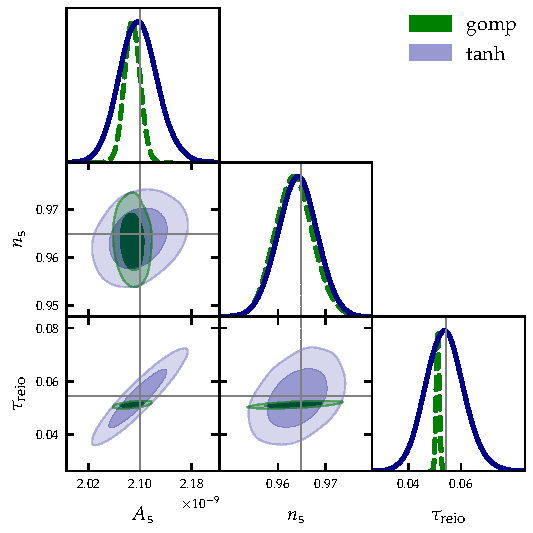
\includegraphics[width=0.6\linewidth]{figs/gomp_tanh_triangle_kill.pdf}
\caption{\textbf{Analysis of CMB data with reionization as a function of
cosmology.}
\YLtodo[inline]{contour and PDFs look quite big}
\paulo{How about now?}
\YL{Can we ``average'' the font sizes of the legend and other texts?}
The green contours represent our results using the Gompertz reionization
model with \cref{eq:SR}, eliminating the need to sample over any
reionization parameter.
The blue contours correspond to the results obtained using the
conventional $\tanh$ model, while the relevant Planck constraints
\cite{Planck2020a} are depicted with gray lines for reference.}
\label{fig:kill}
\end{figure}

\Cref{fig:kill} underscores the impact of our universally-shaped
Gompertz reionization model.
The Gompertz model does not sample over reionization parameters but
maps cosmology parameters to $x_\HI$ profiles.\YL{too many repetitions?}
This approach tightens the constraint on the optical depth to $\approx
1\%$, a remarkable improvement compared to $> 10\%$ with the $\tanh$
prescription.
Furthermore, the constraint on $\As$ improves dramatically since the TT
data is no longer significantly hampered by the degeneracy between $\As$
and $\tau_\reio$.
The error on $\As$ decreases by an impressive factor of 2.5 compared to
Planck's results \cite{Planck2020a}.
Overall, we recover tighter constraints across the board compared to
Planck.
See \Cref{fig:unleashed_gomp} and \Cref{tab:para} in the Extended Data for details.


\section*{Outro}

\begin{figure}[tb]
\centering
\includegraphics[width=\linewidth]{figs/history.pdf}
\caption{\textbf{Reionization history $x_\HI$.}
Our best-fit Gompertz model (green dashed line) of Planck data is
asymmetric and differs significantly from that of the symmetric $\tanh$
model (blue lines, with dotted region representing the 1$\sigma$
errors).
Note $z$ is shown in logarithmic scale of $a^{-1}$.
We also include an alternative mapping from cosmology to Gompertz
timeline in the pink dotted line (see \nameref{ssec:0226}).
Additionally, we include observational constraints from high-redshift
quasars \cite{Greig2017, Banados2018, Davies2018, Greig2019, Wang2020,
Yang2020, Greig2022, Jin2023} and galaxies \cite{Ouchi2010,
Sobacchi2015, Mason2018, Mason2019, Hoag2019, Mesinger2015}.}
\YLtodo[inline]{Unify gomp legend: gomp or Gomp or Gompertz}
\label{fig:history}
\end{figure}

Our results suggest that Planck data favors a delayed reionization
compared to other CMB-based constraints.
Our best-fit cosmological parameters indicate a midpoint of $z_\re =
7.40$ and a duration of $\Delta z \equiv z(x_\HI = 0.05) - z(x_\HI =
0.95) \sim 500 $ Myr.
While our results align with late reionization observations, the
difference from the $\tanh$ model is within 1$\sigma$.
The duration of reionization, though better suited to observational
constraints compared to the $\tanh$ model, might still be considered
somewhat rapid in the context of late reionization scenarios
\cite{Cain2021}.
\Cref{fig:history} illustrates the reionization timeline derived
from our best-fit values.

Our findings for the timeline of reionization align with late
reionization scenarios, which are supported by high-$z$ Lyman-$\alpha$
observations \cite{Keating2020, Cain2021}.
However, recent discoveries by JWST indicate the presence of massive,
bright galaxies at early redshifts $z \sim 10$
\cite{Adams2023, Bradley2023, Donnan2023}.
The presence of these early galaxies suggests a potential preference for
brighter galaxies to drive reionization, a role that in our
\texttt{21cmFAST} simulations was attributed to a population of faint
galaxies.

Furthermore, our results are influenced by the semi-numerical
prescription employed by \texttt{21cmFAST} to ionize the IGM, which,
while efficient and swift, could bias our findings.
Moreover, our exploration within the astrophysical framework of
\texttt{21cmFAST} has been limited to varying the ionization efficiency
(see \nameref{ssec:sims} in the Extended Data).
Therefore, a more comprehensive exploration is warranted to ensure, for
instance, that the rescaling tilt $\tilt$ remains a constant.
Additionally, a valuable exercise to refine the inherent relationship
between cosmological parameters and reionization history would involve
using more realistic, albeit slower, reionization models.
One such option is to use the THESAN simulations \cite{Kannan2022},
which are hydrodynamical simulations incorporating radiative transfer.


\paulo{Around 2000 words.}

\paulo{Body can only have 50 citations.}



\appendix
% extra material limited to 3000 words
\section*{Methodology}
\label{sec:methods}


\subsection*{Simulations}
\label{ssec:sims}

To establish the universality of our proposed Gompertz model for the
neutral hydrogen reionization and its relationship with the cosmological
parameters, we conducted 128 \texttt{21cmFASTv3} simulations to generate
the corresponding $x_\HI(z; \vtheta)$ profiles.
Our parameter space include $\vtheta = \{\sigma_8, \ns, h, \Omegab,
\Omegam, \zetaUV\}$, comprising five cosmological and one astrophysical
parameters.
The selection of $\sigma_8$ instead of $\As$ is imposed by the input
requirements of \texttt{21cmFAST}\footnote{Alternatively, one could use
\texttt{21cmFirstCLASS}\cite{Flitter2024} to avoid $\sigma_8$.}.
We use a scrambled Sobol sequence \cite{Sobol1967, Owen1998} to sample
quasi-uniformly in the $\vtheta$-space, within the following ranges:
%
\begin{alignat}{3}
\label{eq:prior}
\sigma_8 &\in (0.74, 0.90), &\quad
\ns &\in (0.92, 1.00), &\quad
h &\in (0.61, 0.73), \nonumber\\
\Omegab &\in (0.04, 0.06), &\quad
\Omegam &\in (0.24, 0.40), &\quad
\zetaUV &\in (15, 30).
\end{alignat}
%
Their 1D and 2D projections in \Cref{fig:sobol} illustrate the sample
uniformity in parameter space.
Our \texttt{21cmFAST} simulations have a 300 comoving Mpc box size and
$768^3$ ($256^3$) cells for the matter (HI) field.
We maintain most options in their default values and extract the
neutral hydrogen fraction using \texttt{lightcone.global\_xH}.

\begin{figure}[tb]
\centering
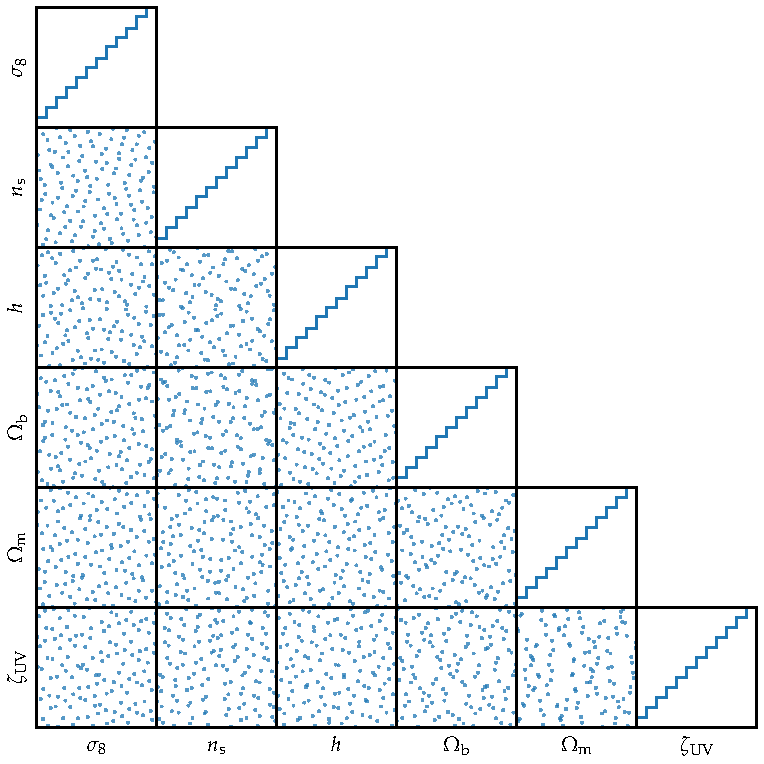
\includegraphics[width=25em]{figs/sobol128.pdf}
\caption{\textbf{Sobol sampling of our $x_\HI$ profiles}, in 6D
parameter space of $\sigma_8$, $\ns$, $h$, $\Omegab$, $\Omegam$, and
$\zetaUV$,
Each point in the lower triangular panels corresponds to the 2D
projection of a \texttt{21cmFAST} run, while the diagonal panels show
the 1D cumulative histograms for each parameter.
These 1D and 2D projections demonstrate the uniformity of our sampling
of the parameter space within the prior range of \cref{eq:prior}.}
\label{fig:sobol}
\end{figure}

The ionization efficiency $\zetaUV$ governs the ability of ultraviolet
photons to escape their parent galaxies and ionize the IGM. An increase
in $\zetaUV$ leads to an earlier completion of HI reionization.
Due to significant uncertainties surrounding $\zetaUV$, we opted to use
a constant value in each simulation.
Note that this choice was made for simplicity, and a more realistic
assumption could be that $\zetaUV$ is a function of halo mass
\cite{Park2019} or redshift.
However, our findings suggest that $\zetaUV$ plays a minor role compared
to the cosmological parameters.
In fact, the best performing symbolic regression expressions (see
\nameref{ssec:pysr} for the selection of best models) do not use
$\zetaUV$.


\subsection*{Helium reionization}
\label{ssec:helium}

The early intergalactic medium is primarily composed by neutral hydrogen
and helium.
Neutral helium (HeI) loses is first electron at the same time as neutral
hydrogen (HI) gets ionized \cite{Trac2007}.
However, there is a second reionization that occurs around $z\sim3$
where Helium (HeII) loses its remaining electron.

CMB photons will scatter off any free electrons, therefore both helium
reionizations contribute to the Thomson optical depth to reionization
$\tau_\reio$, although HeII ionization contribute relatively little in
comparison to HI and HeI ionizations \cite{Liu2016}.

To include the impact of the first helium reionization in our Gompertz
\texttt{CLASS}, we assume it follows that of HI as done in the $\tanh$
model, i.e.\ the free electron fraction $x_\e$ is given by
%
\begin{align}
\label{eq:xe_H_He}
x_\e
&= \Bigl(1 + \frac{n_\He}{n_\mathrm{H}} - x^\rec_\e\Bigr) x_\e^\gomp
  + x^\rec_\e
\nonumber\\
%
&= \Bigl(1 + \frac{Y_\He}{C (1 - Y_\He)} - x^\rec_\e\Bigr) x_\e^\gomp
  + x^\rec_\e,
\end{align}
%
where $n_\He / n_\mathrm{H}$ is the helium to hydrogen number density
ratio, $C \equiv m_\He / m_\mathrm{H} \approx 4$ is their mass ratio,
$Y_\He$ is the helium mass fraction, $x_\e^\gomp$ corresponds to the
contribution of free electrons due to \cref{eq:uni}, and $x^\rec_\e
\approx 10^{-4}$ is the leftover free electrons from after
recombination.

Given the relatively small impact of the HeII reionization on
$\tau_\reio$, the current uncertainties regarding its timeline, and the
difficulty involved with its accurate modeling \cite{Hotinli2023,
Upton2020}, we opt to follow the conventional approach and include the
second Helium reionization using the $\tanh$ model
%
\begin{equation}
\label{eq:xe_tot}
x_\e^\mathrm{Tot} = x_\e + \frac{Y_\He}{2C(1 - Y_\He)}
  \biggl(\tanh{\Bigl(\frac{z_\re^\HeII - z}{\Delta z^\HeII}\Bigr)} + 1\biggr),
\end{equation}
%
where $z_\re^\HeII = 3.5$ and $\Delta z^\HeII = 0.5$ are the midpoint
and duration of the second helium reionization, respectively.
These choices are also the default values used by \texttt{CLASS}.


\subsection*{Shape universality and modeling}
\label{ssec:shape}

\begin{figure}[tb]
\centering
\includegraphics[width=0.6\linewidth]{figs/shape_6.pdf}
\caption{\textbf{Universal shape of $x_\HI$.}
\emph{(Top)} 128 simulated $x_\HI$ timelines (thin light gray lines)
exhibit universality, after power-law transformations $\ar =
(a/\ap)^\tilt$.
The blue curves in all panels show our fitted analytic shape model, a
composition of the Gompertz curve with a 5th-degree polynomial in
\cref{eq:uni,eq:poly}.
\emph{(Middle)} Time derivative of $x_\HI$, can be interpreted as a PDF
if we view $x_\HI$ itself as the CDF.
We first discovered the universality by translating and rescaling each
$x_\HI$ using the mean and variance of its PDF, though now switch to the
better approach that jointly fits the global shape and individual
power-law parameters.
We use the latter as target of symbolic regression.
\emph{(Bottom)} Timelines transformed by the inverse of Gompertz
function, modeled in blue curve with a 5th-degree polynomial in
\cref{eq:poly}.}
\label{fig:shape}
\end{figure}

We discovered the universality in the shape of $x_\HI$ timelines before
attempting to build analytic model for it.
Because $x_\HI$ varies monotonically between 1 and 0, we can view it as
a CDF and derive its PDF, with which we can weigh the logarithmic scale
factor $\ln a$ to compute its mean and standard deviations.
It was immediately obvious to us that the $x_\HI$'s had a common shape
to percent level, after translation by their means and rescaling by
their standard deviations.
However, given our broad parameter range in \cref{eq:prior}, some
$x_\HI$'s have not reached 0 by the end of simulations, resulting in
imperfect transformations hurting the universality.

To address this, we construct flexible models for the universal shape,
and fit it jointly with individual transformation parameters of each
$x_\HI$ timeline.
We compose the Gompertz function $\gomp$, defined in \cref{eq:uni}, with
a low-degree polynomial $P_m$, where $m = 1, 3, 5, 7$ progressively.
We fit the composed shape to minimize the mean squared error (MSE) in
128 $x_\HI$'s and at 92 time points in each, and find the objective
value improve with $m$ but only marginally from $P_5$ to $P_7$.
Therefore, our final shape model is a composition of $\gomp$ and $P_5$,
(see the lower panel of \Cref{fig:shape}), and has 6 parameters to fit.

As for the transformation parameters, as in the PDF approach, we use an
affine transformation $\ln\ar = \tilt (\ln a - \ln\ap)$, or equivalently
a power law in \cref{eq:map}.
Because each $x_\HI$ has its own parameters of $\ap$ and $\tilt$, we
have in total $262 = 6 + 2 \times 128$ parameters to determine in the
joint fit.
\Cref{fig:shape} shows all 128 $x_\HI$ timelines and their universality
after transformations.
We can then use the fitted $\ap$ and $\tilt$ as the target for symbolic
regression, to model their cosmological dependences on the other
independent parameters.


\subsection*{Symbolic regression}
\label{ssec:pysr}

\begin{figure}[tb]
\centering
\includegraphics[width=0.8\linewidth]{figs/pareto.pdf}
\caption{\textbf{Pareto front for symbolic regression} (blue solid
steps) illustrates the trade-off between regression accuracy and
expression complexity.
We further add the lower convex hull to aid model selection: each
segment of the orange dotted line represents a power-law trade-off in
this log-log plot, and every model that touches the convex hull is more
economic -- in the sense of accuracy gain at cost of complexity -- than
the nearby models above the segments.
As an example, here we show the results of $\ln\ap(\vtheta)$, where the
complexity 11 point gives \cref{eq:SR}.}
\label{fig:pareto}
\end{figure}

SR learns a model of data in the form of analytic expressions.
Unlike traditional fittings that are restricted by their specific
parameterization, SR searches in the vast function space of all
expressions composed of specified operations, input variables, and free
constants.
It is NP-hard \cite{SongEtAl2024, VirgolinPissis2022} and typically need
genetic or deep learning-based algorithms.
In this work, we use the \texttt{PySR} package \cite{Cranmer2020b,
Cranmer2023} which performs SR optimizations using a multi-population
genetic algorithm.
%\YLtodo[inline]{Miles, it'd be great if you can refine/rewrite the SR
%and PySR intro}

With \texttt{PySR}, we search for symbolic expressions that take the 6
parameters in \Cref{fig:sobol} as inputs and output $\ln\ap$ or $\tilt$,
to minimize the MSE loss.
Here, the search space is the set of expressions composed of 5 binary
operators ($+$, $-$, $\cdot$, $/$, and power function) and 2 unary
operators ($\exp$ and $\ln$).
Each expression naturally takes the form of a binary tree, and the
total number of nodes is a measure of its complexity.
We use 512 \texttt{PySR} populations each having 33 expressions, and
optimize for 10000 iterations each with 10000 cycles.
%\YLtodo[inline]{Miles, could you translate this into some brief
%description in the language of evolve-simplify-optimize loop, mutation,
%crossover, and tournament?}

More complex expressions tend to fit more accurately, a trade-off
typically visualized by the Pareto front, as shown in \Cref{fig:pareto}.
Better and more economic expressions can achieve a lower loss at
moderate increase of complexity.
To aid model selection, we use a heuristic that compares all expressions
on the Pareto front globally, and only considers models that fare
favorably in power-law trade-offs of the form
%
\begin{equation}
\mathrm{loss}^{1 - \gamma} \cdot \mathrm{complexity}^\gamma
= \mathrm{const}, \quad \forall \gamma \in (0, 1).
\end{equation}
All such expressions lie on the lower convex hull of the Pareto front,
as illustrated in \Cref{fig:pareto}.

For the pivot $\ln\ap$, we find complexity 11 is enough for the MSE loss
to reach $10^{-4}$ (sub-percent level error on average), so there's no
need to use expressions more complex that that.
However, for the tilt $\tilt$, complexity 1, i.e.\ a constant, fit with
a loss $\approx 0.1$ ($4\%$ error on average), while higher complexities
can help but very slowly.
Therefore, based on the economic heuristic, we choose expressions of
complexity 11 and 1, for $\ln\ap$ and $\tilt$, respectively.

This preference for constant tilt could be a consequence of the
astrophysical assumptions of reionization in \texttt{21cmFAST}.
A more complex simulation, such as one involving radiative transfer or
different X-ray preheating \cite{Montero2024}, might reveal a different
tilt.

\begin{table}[t]
\centering
\caption{\textbf{Parameter constraints from Planck CMB data.}
Summary table of the constraints for representative parameters of the
universal shape (Gompertz) and $\tanh$ reionization models.
The constraints use CMB `TTTEEE' + lensing information.
The results from Planck analysis \cite{Planck2020a} are included for
comparison.
The validation models are gomp 0 and $\tanh$ 0, gomp 0 does not include
the cosmological information present in the timeline of reionization.
In contrast, gomp 1, and the alternative mapping gomp 2, both include
the additional cosmological dependence in the reionization timeline.
The shaded cells highlight the parameters that are sampled over by MCMC
for the different models.
The numbers in parentheses give the marginalized 1$\sigma$ uncertainty
in the last two significant digits.
We highlight the best constraints in boldface, with improvements by
factors of 12 and 2.5 on $\tau_\reio$ and $A_s$, respectively.
The age of the Universe and $H_0$ are in unit of Gyr and km/s/Mpc,
respectively, and $S_8 \equiv \sigma_8 \sqrt{\Omegam/0.3}$ as usual.}
\makebox[\textwidth][c]{\footnotesize
\renewcommand{\arraystretch}{1.3}
\begin{tabular}{c *{3}{r} !{\hspace{.5em}} *{3}{r}}
\toprule
 & \multicolumn{3}{c}{Gompertz reionization} & \multicolumn{3}{c}{Tanh reionization} \\
\cmidrule(lr){2-4} \cmidrule(lr){5-7}
Parameter & gomp 0 & gomp 1 & gomp 2 & $\tanh$ 0 & $\tanh$ 1 & Planck PR3\cite{Planck2020a} \\
\midrule
$10^{9} \As$ & \sampled 2.101(31) & \textbf{2.088(12)} & \textbf{2.089(13)} & \sampled 2.099(30) & 2.098(30) & \sampled 2.100(30) \\
$\ns$ &\sampled 0.9638(41) & \sampled 0.9634(40) & \sampled 0.9634(40) & \sampled 0.9641(42) & \sampled 0.9641(41) & \sampled 0.9649(42) \\
$\Omegac h^2$ &\sampled 0.1201(12) & \sampled 0.1203(11) & \sampled 0.1202(11) & \sampled 0.1201(12) & \sampled 0.1201(12) & \sampled 0.1200(12) \\
$\Omegab h^2$ & \sampled 0.02235(15) & \sampled 0.02233(14) & \sampled 0.02233(14) &  \sampled 0.02235(15) & \sampled 0.02235(15) & \sampled 0.02237(15) \\
$\Omegam$ & 0.3157(76) & 0.3171(68) & 0.3168(68) & 0.3157(76) & 0.3159(75) & 0.3153(73) \\
$\Omegam h^2$ & 0.1430(11) & 0.1433(10) & 0.1432(10) & 0.1430(11) & 0.1431(11) & 0.1430(11) \\
$\OmegaL$ & 0.6842(76) & 0.6828(68) & 0.6831(68) & 0.6842(76) & 0.6840(75) & 0.6847(73) \\
Age & 13.800(23) & 13.803(20) & 13.803(22) & 13.800(23) & 13.800(23) & 13.797(23) \\
$H_0$ & 67.32(55) & \sampled 67.22(49) & \sampled 67.24(50) & 67.32(55) & \sampled 67.31(54) & 67.36(54) \\
$100 \theta_\mathrm{X}$ & \sampled 1.04184(29) & 1.04183(29) & 1.04183(29) & \sampled 1.04815(29) & 1.04184(29) & \sampled 1.04092(31) \\
$\sigma_8$ & 0.8109(59) & \sampled 0.8092(45) & \sampled 0.8092(46) & 0.8108(60) & \sampled 0.8105(59) & 0.8111(60) \\
$S_8$ & 0.832(13) & 0.832(13) & 0.832(13) & 0.832(13) & 0.832(13) & 0.832(13) \\
$\tau_\reio$ & \sampled 0.0546(76) & \textbf{0.05115(61)} & \textbf{0.05140(63)} & \sampled 0.0543(75) & 0.0538(74) & \sampled 0.0544(73) \\
$z_\re$ & 6.81(68) & 7.40 & 7.41 & 7.67(75) & \sampled 7.62(74) & 7.67(73) \\
\bottomrule
\end{tabular}}
\label{tab:uber-table}
\end{table}

\begin{figure}[t]
\centering
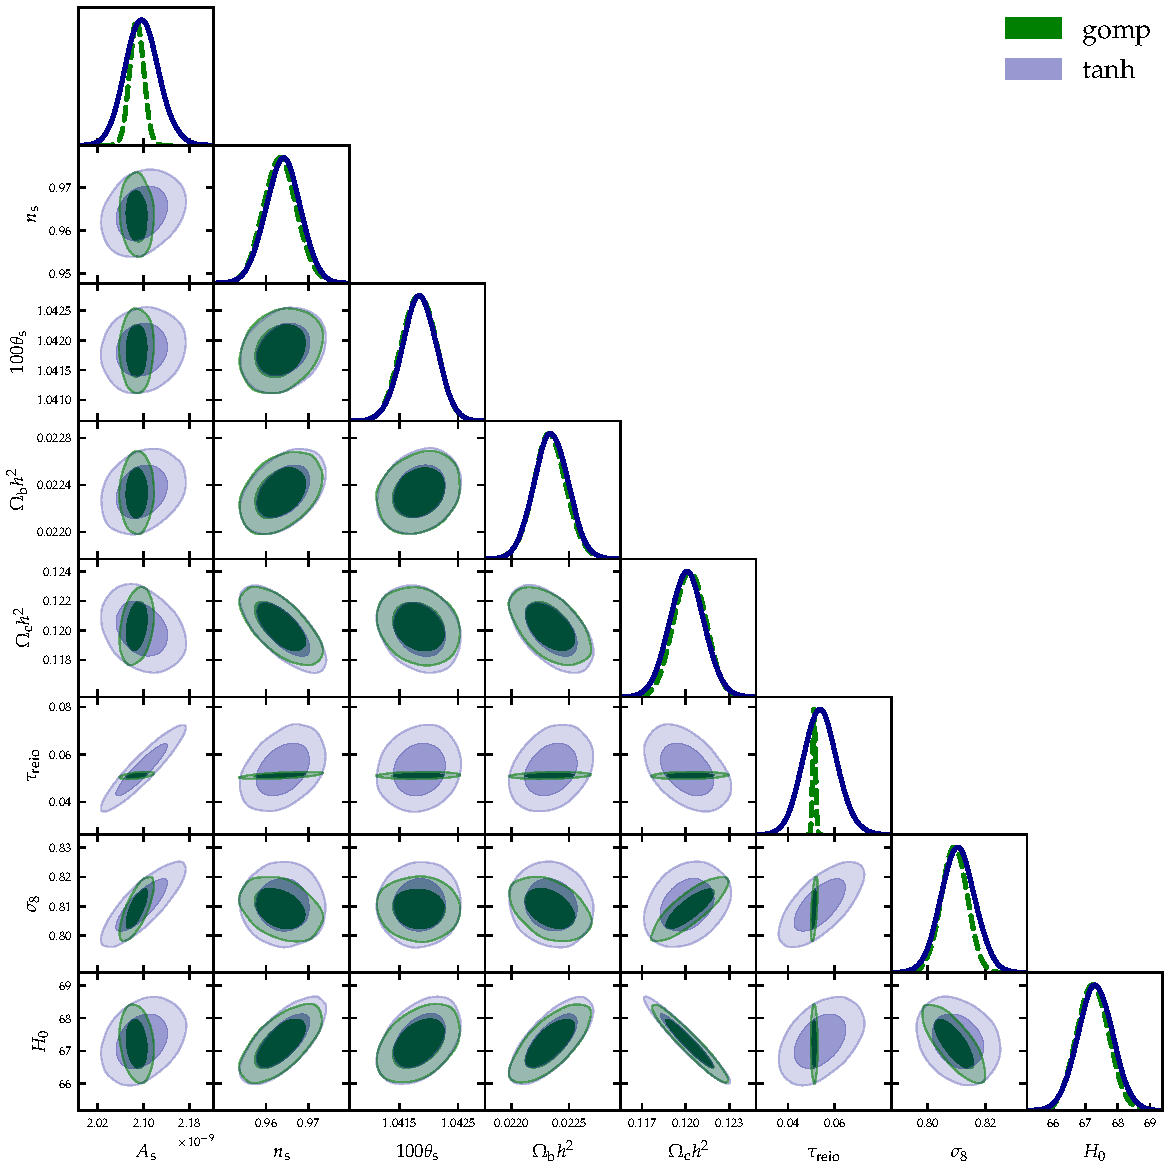
\includegraphics[width=\linewidth]{figs/gomp_tanh_triangle_kill_full.pdf}
\caption{\textbf{Analysis of CMB data treating $\tau_\reio$ as a derived
parameter using \cref{eq:uni,eq:poly,eq:map,eq:SR} vs.\ sampling it with
the conventional $\tanh$ model.} Here gomp 1 combines our Gompertz universal
shape with the rescaling pivot and tilt obtained via symbolic regression. Note that for
gomp 1 we do not sample over $z_\re$ since \cref{eq:uni} does not depend on it.
The green (blue) contours correspond to the constraints obtained with
our Gompertz universal shape ($\tanh$ 1 model).}
\label{fig:unleashed_gomp}
\end{figure}

\begin{figure}[t]
\centering
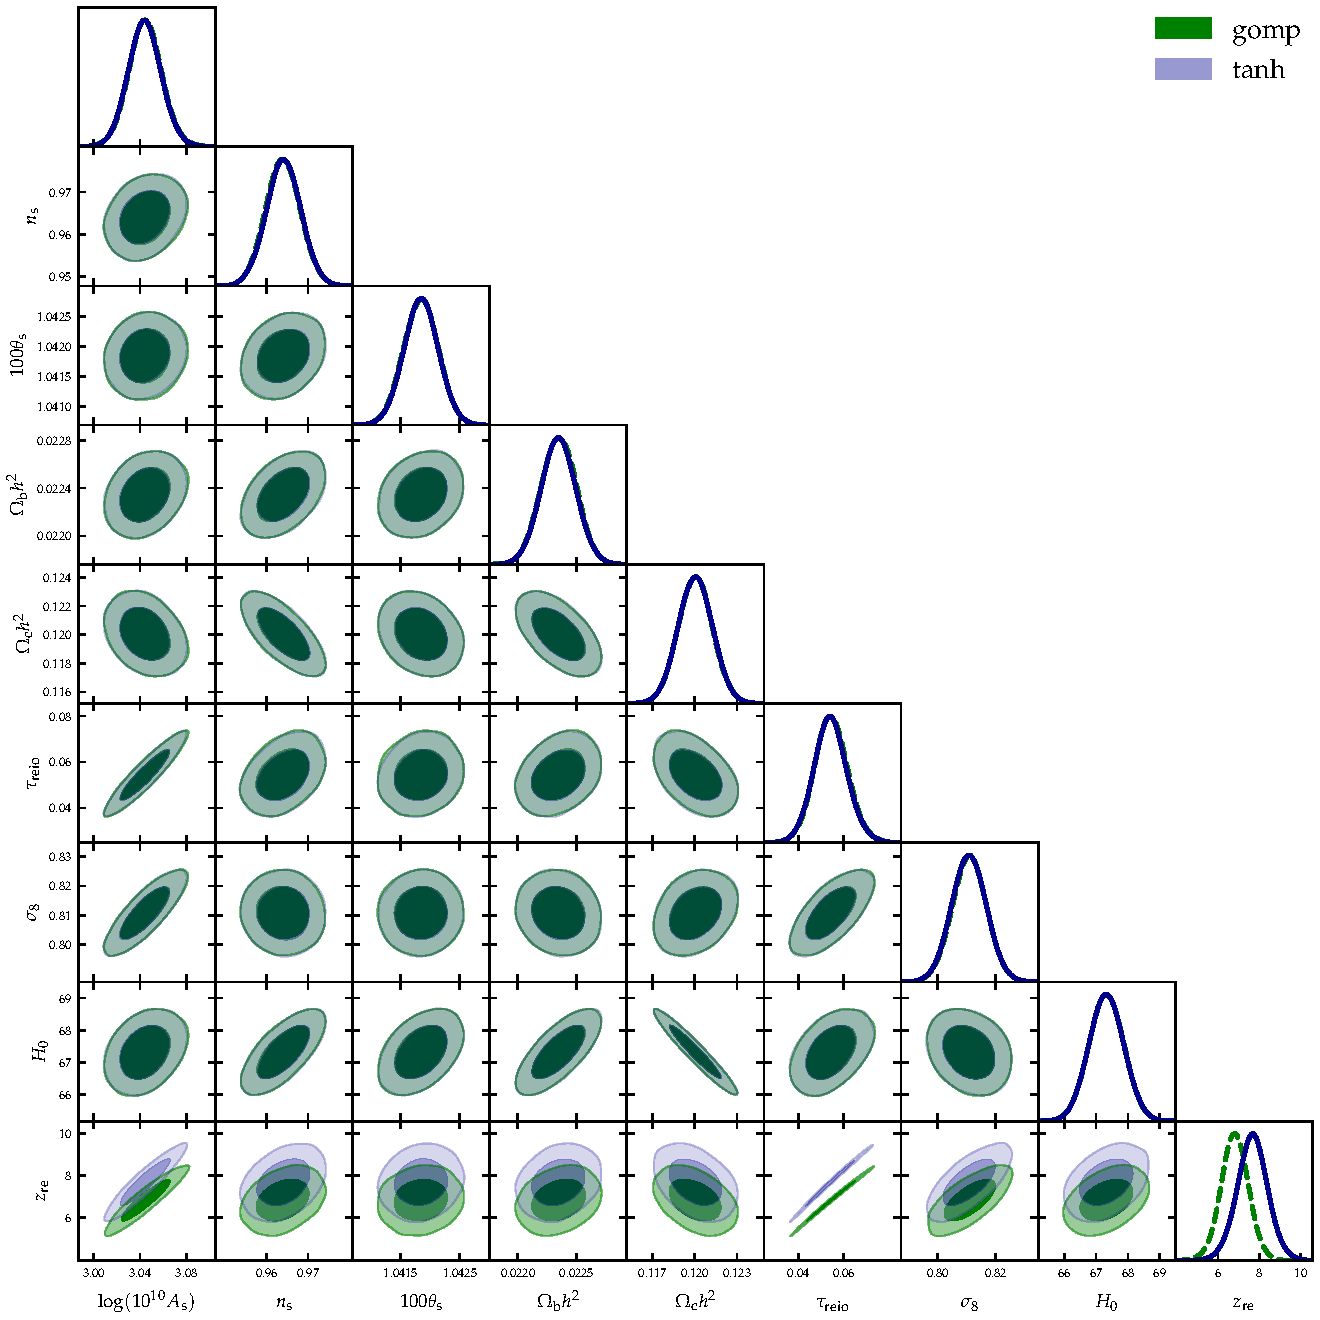
\includegraphics[width=\linewidth]{figs/gomp_tanh_triangle_tau.pdf}
\caption{\textbf{Validation of our universal shape for $x_\HI$ in \cref{eq:uni,eq:poly} vs.\ the
conventional $\tanh$ model using CMB data with sampling over $\tau_\reio$.}
Note that we have not \emph{eliminated} $\tau_\reio$ from the analysis
yet. Here, we use the standard choice of sampling
over optical depth and obtain the corresponding reionization history via bisection.
The green (blue) contours correspond to the constraints obtained with
our gomp 0 ($\tanh$ 0) model.}
\label{fig:tg}
\end{figure}


\subsection*{Alternative mapping}
\label{ssec:0226}

The mapping between neutral hydrogen profiles and cosmology is not
unique.
This is because symbolic regression algorithms can be non-convergent.
Moreover, the resulting symbolic expressions can depend on the data used
for training, i.e.\ overfitting.

To investigate the impact of overfitting, we train an alternative
mapping of reionization with cosmology using only half of the
\texttt{21cmFAST} $x_\HI$ profiles, which we refer as gomp 2.
For the tilt, once again we find a constant $\tilt = 8.331$, remarkably
close to the value obtained using the full simulated data (8.290).
And for the pivot, we obtain
%
\begin{equation}
\label{eq:SR0226}
\ln\ap(\vtheta) = (1.039 + \sigma_8) (\Omegab - \Omegam h - \ns),
\end{equation}
%
with a training loss of $1.2 \times 10^{-4}$.
Now we can test this on the other half of our $x_\HI$ sample and get a
validation loss of $1.4 \times 10^{-4}$, only slightly larger than the
training loss implying we are safe from overfitting.

Unsurprisingly, \cref{eq:SR0226} recovers the cosmological trends
present in \cref{eq:SR}.
Specifically, increasing $\ns$, $\Omegam$, and $\sigma_8$ leads to an
earlier reionization scenario, while a higher value of $\Omegab$
slightly delays reionization.
Furthermore, the impact of the Hubble constant is once again linked to
the matter density, albeit not in the same manner as in
\cref{eq:SR}.
This is likely evidence that the role of $h$ is limited, and
\texttt{PySR} considers its influence in conjunction with $\Omegam$
without increasing the complexity of the analytic expression.

Replacing \cref{eq:SR} with \cref{eq:SR0226}, we rerun the analysis
following the same approach, and summarize the results in
\Cref{tab:uber-table}.
Comparing these findings to our previous results, we observe strikingly
similar values for all cosmological parameters, albeit with smaller
deviations from the Planck results.
The consistency between our results using the full $x_\HI$ sample and
those using only half of it indicates that our symbolic expression
mappings perform robustly and are not biasing the parameter inferences.


\subsection*{MCMC inference}
\label{ssec:fits}

\Cref{tab:uber-table} summarizes the results obtained by performing MCMC
Bayesian inference with \texttt{Cobaya} for the models considered
throughout this work.
We also include the Planck results \cite{Planck2020a} for reference.
In total, we run three Gompertz reionization and two $\tanh$
reionization models, where $\tanh$ 0, Planck PR3, and gomp 0 sample over
the typical 6 cosmological parameters (see shaded parameters in
\Cref{tab:uber-table}).
In contrast, gomp 1, and gomp 2 sample over $\vtheta = \{\sigma_8, \ns,
\Omegab h^2, \Omegac h^2, h\}$.
Similarly, $\tanh$ 1 samples over the same parameters as gomp 1 but with
the inclusion of $z_\re$, and agrees with $\tanh$ 0 as the expected
result from this sanity check.

There is an apparent discrepancy between the different models in
$\theta_\mathrm{x}$, a proxy for the angular scale of the acoustic
oscillations ($\theta_*$).
The difference is due to our use of $100\theta_\mathrm{s}$, which
corresponds to the peak scale parameter defined exactly as the
ratio of the sound horizon divided by the angular diameter at
decoupling, with decoupling time given by the maximum of the visibility
function, i.e.\ the standard choice for CLASS.
In contrast, the Planck collaboration reports $100\theta_\mathrm{MC}$,
which is given by Eq.~(6) in \cite{Planck2014}, and corresponds to the
standard choice in \texttt{CosmoMC}\cite{Lewis2002}.

Although \Cref{tab:uber-table} does not display an error in the midpoint of
reionization in the gomp 1 and gomp 2 models, it is important to note that an error
does exist. Unfortunately, it cannot be automatically computed with \texttt{Cobaya} because
gomp 1 and gomp 2 do not sample over reionization parameters. Therefore,
$z_\re$ has no meaning in our Gompertz \texttt{CLASS}\footnote{This oversight
can be corrected; however, it would require re-running the chains.} for models
that take advantage of \cref{eq:premise}.

Remarkably, the inferred value of $S_8$ remains consistent across all reionization
models, even when $\sigma_8$ and $\Omegam$ vary between models. This trend
suggests that different reionization models neither alleviate nor exacerbate the $S_8$
tension. While this observation holds for the Planck PR3 data, we anticipate that
incorporating low-redshift Baryon Acoustic Oscillation (BAO) data may affect this
conclusion. Future work will explore the implications of Gompertz reionization
for the joint analysis of CMB and low-redshift data.


\FloatBarrier



\paragraph{\large Supplementary information} No.

\paragraph{\large Acknowledgements}
This work is supported by The Major Key project of PCL.
The authors acknowledge PCL's Cloud Brain for providing computational
and data storage resources that have contributed to the results reported
within this paper.

\section*{Declarations}
% If going for Nature astronomy, then we should include here a bunch of required declarations. Most of them will be "NA"...

\paragraph{\large Authors contributions}
P.M.C.\ and Y.L.\ contributed equally to all stages of the project.
M.C.\ contributed to the implementation of the symbolic regression
algorithm.

\vspace{-1em}
\paragraph{\large Correspondence and requests for materials}
Should be addressed to Paulo Montero-Camacho and Yin Li.

\vspace{-1em}
\paragraph{\large Code availability}
The paper source files and the scripts used in this work are available
at \href{https://github.com/eelregit/5par}{\faGithub}.

\vspace{-1em}
\paragraph{\large Funding}
Not applicable.

\vspace{-1em}
\paragraph{\large Competing interests}
The authors declare no competing interests.

\vspace{-1em}
\paragraph{\large Ethics approval}
Not applicable.

\vspace{-1em}
\paragraph{\large Consent to participate}
Not applicable.

\vspace{-1em}
\paragraph{\large Consent for publication}
Not applicable.
 % will change this to include all others declarations that are required.


\bibliographystyle{JHEP}
{\singlespacing
\bibliography{main}
}


\end{document}
